\section{Source analysis, scope, and reproducibility}
\label{sec:provenance}

\subsection{What was checked in the Lean development}

The source analysis used the fixed ProveIt commit cited in
Section~\ref{sec:overview}, rather than the changing branch name
\texttt{main}. The vendored \texttt{grh/} tree has Git tree identifier
\begin{quote}\small\ttfamily
2e133df63d7f4da6b3059c4195324f8e9187ba73.
\end{quote}
All 818 files in
the inspected copy matched their Git blob identifiers in the remote
tree; the complete record is in \path{provenance/lean_file_manifest.json}.
There are 803 Lean source files under \texttt{src/}; a static
import walk from \texttt{Main} reaches all 803. These are provenance
and dependency checks, not a manual verification of every proof line.

The exported interface uses ordinary Mathlib definitions. In
particular, \texttt{riemannHypothesis} has type
\texttt{RiemannHypothesis}. The Dirichlet interface proves nonvanishing
to the right of $1/2$ with the principal pole excluded, and then the
critical-line statement for zeros in the open critical strip. This
includes imprimitive characters; it does not assert GRH for all
automorphic or Artin $L$-functions. The pinned toolchain is Lean
\texttt{v4.35.0}, with Mathlib revision
\texttt{56a005855ea17e0b0958f73ec801ae140b0a1679}.

A comment- and string-aware source scan found no active occurrence of
\texttt{sorry}, \texttt{admit}, \texttt{axiom}, \texttt{unsafe},
\texttt{native\_decide}, \texttt{run\_cmd},
\texttt{ofReduceBool}, or \texttt{addDecl} in that source tree.
The intentionally incomplete challenge file is outside the imported
tree. No new full Lean build or external-checker replay was performed
for this report. The separate verification page~\cite{Sutherland}
reports completed checks of the upstream theorem statements; that
evidence is distinct from the source inspection performed here.

The analytic chain has a useful modular structure. The interface
\texttt{New.IsPolar.landau} turns a one-sided bound on a prime
remainder into the absence of poles of its Laplace transform. The
residue computation in
\texttt{New.isPolar\_primeRemainder} initially produces a difference
of untwisted and quadratic-twisted zero multiplicities. A twist is
chosen that has no zeros in a prescribed finite-height box. The
remaining multiplicities are nonnegative, so the Landau conclusion
forces them to vanish individually. The final bound feeds this
criterion into \texttt{New.grh}. The chosen twist depends on the
box; the source does not require a single twist to work at every
height.

The geometric part also exposes stronger information than a
determinant identity: it proves normalized operator identities of
the form $\Theta^*\Theta=cR$ and their chain analogues. The scalar is
stated as complex, so positivity of an unnormalized factor cannot be
inferred without its phase. This is a potential route to other
extensions, but it is not an input to the probability theorems proved
here. The detailed audit and source identifiers are supplied in
\path{evidence/lean_source_audit.md}.

\subsection{Article dependency and novelty comparison}

The directly used part of the article is
\path{Article/sections/ana.tex}, with Git blob identifier
\begin{quote}\small\ttfamily
6b414e43f44bd89c5a7fce0c0f2a0cf08626cc8b.
\end{quote}
The dependency consists of two results in \texttt{ana:sec:smalldev}:
the gamma series and its scalar lower-tail asymptotic.
All 21 inspected section files matched
their pinned Git identifiers. The article is a merged collection of
research reports, not itself a Lean formalization. This report
reproves the needed probability statements from the spectral counting
assumption, so its new results do not depend on trusting all other
claims in that collection.

The seven incoming archives present at the inspected snapshot were
also matched by Git blob identifiers and checked for related material.
Their names and matches are recorded in
\path{provenance/incoming_overlap_check.json}. The overlap search was
a targeted text-and-topic review, not an exhaustive comparison of
every possible equivalent theorem.

\begin{table}[htbp]
\centering\small
\begin{tabular}{@{}>{\raggedright\arraybackslash}p{0.29\textwidth}>{\raggedright\arraybackslash}p{0.65\textwidth}@{}}
\toprule
Prior input & Contribution or distinction in this report\\
\midrule
Reciprocal completed-function laws; Hadamard products
\cite{RoynetteYor,GaoHannigLeeTorcaso}
& The random series and its transform are inputs; they are not claimed
as discoveries here.\\[5pt]
Scalar lower tails in the supplied article~\cite{ProveItArticle}
& Theorem~\ref{mc:thm:joint} determines the conditional allocation,
fluctuations, boundary slack, and low coordinates jointly.\\[5pt]
Gibbs conditioning and small Gaussian norms
\cite{CampenhoutCover,MayerWolfZeitouni}
& Theorem~\ref{mc:thm:threshold} treats an increasing number of
coordinates in total variation and computes the sharp transition.\\[5pt]
Weighted conditional bridges~\cite{SobolevShklyaev}
& A spectral clock and exact centering are identified. No general
priority claim for conditional Brownian bridges is made.\\[5pt]
Tilted reciprocal-$\xi$ asymptotics~\cite{Sra}
& The equal-rate and unequal-rate block transitions are distinguished;
Theorem~\ref{med:thm:height} resolves the half-contribution height.\\
\bottomrule
\end{tabular}
\caption{Scope of the extension relative to the main sources checked.}
\end{table}

The targeted search covered combinations of reciprocal $\xi$ laws,
small deviations of gamma sums, conditional Gaussian bridges,
equivalence of ensembles, growing coordinate blocks, and
total-variation thresholds. It located the related work in the
bibliography but not the precise statements proved here. The honest
novelty claim is a proved extension not located in the inspected
materials and targeted literature search. Publication priority over
all literature has not been established.

\subsection{Analytical review and numerical illustrations}

A separate model-assisted review checked the written proofs for the conditional
density normalization, the Fourier bounds, the growing-block
likelihood, both transition constants, and the median-height
centering. Review notes are included in the archive. These are
mathematical reviews, not external refereeing or machine proof certificates. In particular,
the new theorems have not been added to the Lean project.

The reproducible script \path{code/verify_and_illustrate.py} uses seed
\texttt{20261127}. The recorded run used Python 3.12.14, NumPy 2.3.5,
SciPy 1.17.0, mpmath 1.3.0, and Matplotlib 3.10.8. It performs three
different checks, whose meanings should be kept separate.

First, numerical quadrature at 60 decimal digits checks $C_1$ and
$C_2$ at four different pairs $(\alpha,p)$, with numerical
discrepancies below $10^{-20}$. The implicit median equation is solved
at $\ell=2,4,8,16,32,64$, with residuals below $10^{-50}$. These are
high-precision floating-point checks; the identities and existence
claims are established by the analytical proofs above.

Second, the script simulates the explicitly finite model
$\gamma_j=j$, $1\le j\le4096$, with $\theta=1$. This is not the
zeta spectrum. At $u=32$ and $128$, it draws 50,000 samples from the
tilted independent exponentials and accepts a sample with probability
\[
 \mathbf1_{\{S\le x\}}\exp\{u^2(S-x)\}.
\]
The resulting accepted samples have exactly the conditional law of
the specified finite original sum. There were 3,935 and 1,931
acceptances, respectively. The observed mean boundary slack was
$0.9564$ and $0.9911$, against its limiting value one. At cutoff
$c=1$, the observed centered variance was $0.1622$ and $0.1525$,
against the limiting bridge variance
$1/4-1/\pi^2\simeq0.14868$.

\begin{figure}[htbp]
 \centering
 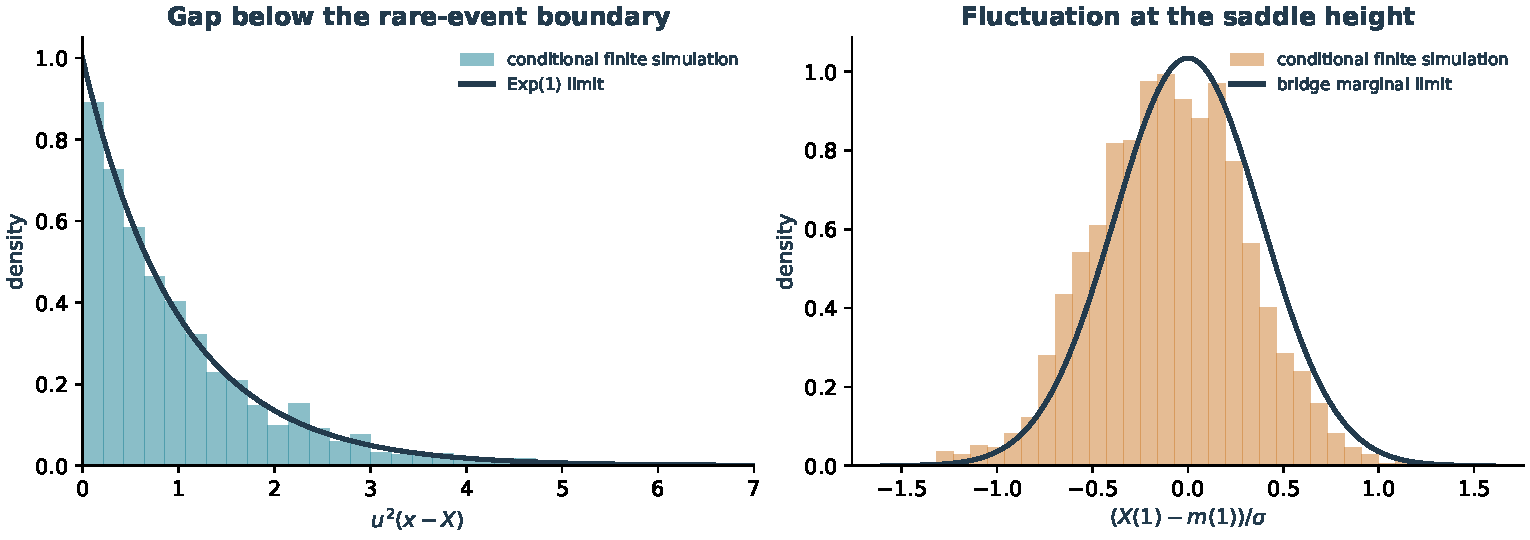
\includegraphics[width=\textwidth]{figures/finite_model_simulation.pdf}
 \caption{A finite synthetic-spectrum illustration at $u=128$.
 The solid curves are asymptotic limits, not fitted distributions.
 The data are not zeta-zero simulations.}
\end{figure}

These finite simulations do not establish asymptotic independence.
For example the correlation of the $c=2$ fluctuation with the boundary
slack is still approximately $-0.443$ at $u=128$. Such finite-saddle
effects remain visible and are reported in the raw data rather than
suppressed.

Third, a separate likelihood experiment compares the two independent
gamma products appearing in Theorem~\ref{mc:thm:threshold}. Its
synthetic points are
\[
 \widetilde\gamma_j=\frac{2\pi j}{W(j/e)},
\]
where $W$ is the principal Lambert function. They have the desired
Riemann--von Mangoldt counting asymptotic, but are not actual zeta
zeros. An exact likelihood-ratio event gives the Monte Carlo
total-variation estimate, using 50,000 draws for each row below.

\begin{table}[htbp]
\centering\small
\begin{tabular}{@{}rrrrrr@{}}
\toprule
$u$ & $c$ & Coordinates & TV estimate & Standard error & Limit in
\eqref{eq:overview-TV}\\
\midrule
1,000 & 1 & 62 & 0.04740 & 0.00095 & 0.06359\\
1,000 & 2 & 162 & 0.28110 & 0.00201 & 0.34826\\
1,000 & 3 & 277 & 0.67968 & 0.00209 & 0.78642\\
10,000 & 1 & 661 & 0.05080 & 0.00098 & 0.06359\\
10,000 & 2 & 1,546 & 0.30354 & 0.00206 & 0.34826\\
10,000 & 3 & 2,516 & 0.72354 & 0.00200 & 0.78642\\
\bottomrule
\end{tabular}
\caption{Finite product comparisons at
$h=c(u^4/\log u)^{1/5}$. The theorem does not supply a finite-$u$
error bound, and logarithmic convergence is slow.}
\end{table}

The differences from the limiting curve are appreciably larger than
Monte Carlo uncertainty. Even replacing the limiting parameter by
the exact finite sum $\tau_u^2$ need not eliminate the discrepancy:
at $(u,c)=(10{,}000,3)$ its Gaussian profile is about $0.73762$.
The numerical experiment illustrates the approach to the transition;
it is not a certified approximation for finite saddles.

\begin{figure}[htbp]
 \centering
 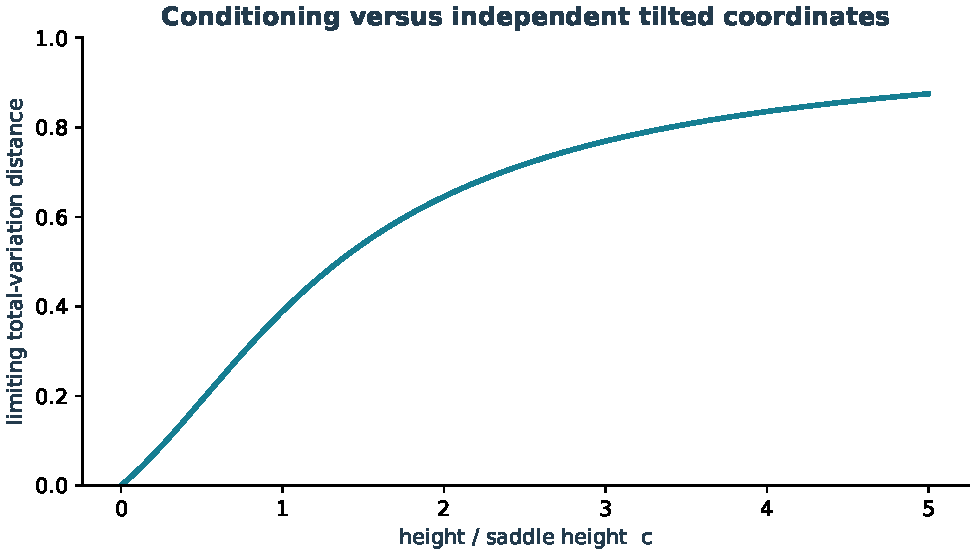
\includegraphics[width=0.78\textwidth]{figures/ensemble_transition.pdf}
 \caption{The separate transition for independence with the actual
unequal rates: the analytic function $D(V(c))$ from
Theorem~\ref{mc:thm:macroscopic}.}
\end{figure}

\subsection{Files and reproduction}

The archive contains this PDF, the complete \LaTeX{} sources, the
Python script, all figures in PDF/PNG format,
the numerical JSON output, source manifests, and review notes.
\path{README.md} explains the contents and commands;
\path{code/build_report.sh} rebuilds the PDF using \texttt{latexmk}.
The existing figures suffice to compile the manuscript, so rebuilding
it does not require repeating the simulation.

All conclusions concern explicitly defined random weights attached to
deterministic zero ordinates. They imply neither randomness of the
zeros nor a zero-spacing, pair-correlation, simplicity, or linear
independence theorem. Fixed conductors and fixed finite products are
allowed; no uniform result in a growing conductor or degree is claimed.
The general regular-variation theorem is unconditional. RH or
Dirichlet GRH supplies the exact completed-function interpretation
in the arithmetic applications.

